%!TEX encoding=UTF-8 Unicode
\section{Motivations}
\label{sec:motivations}

\subsection{Intro}
\label{sec:motivations-intro}

Importance of Mapping:
\begin{itemize}
    \item First touch
    \item Interleave
\end{itemize}

Why Not automated tools
\begin{itemize}
    \item Trainning time
    \item Garbage in/ garbage out (matrix modulo / bloc)
\end{itemize}
\subsubsection{Matrix multiplication}

\DB{Rewritte}

Our first benchmarks is a matrix multiplication ($C=A*B$), we use it to show he
impact of both manual mapping and original quality of the code. We compare two
implementations of the matrix multiplication, in first one, called
\emph{Naive}, each threads start by computing $C[0][tid]$ and then jumps $N$
elements after in the matrix, where $N$ is the number of threads. Although
this implementation is known to be bad, comparing how much it's accelerated by
the best mechanism to the acceleration of a better version to understand the
importance of the quality of the original code. \DB{Rewritte later.} The
second implementation is a bloc matrix multiplication (not recursive).

\begin{figure}[htb]
    \centering
    \subfigure[Structure A (naive)]{
        % 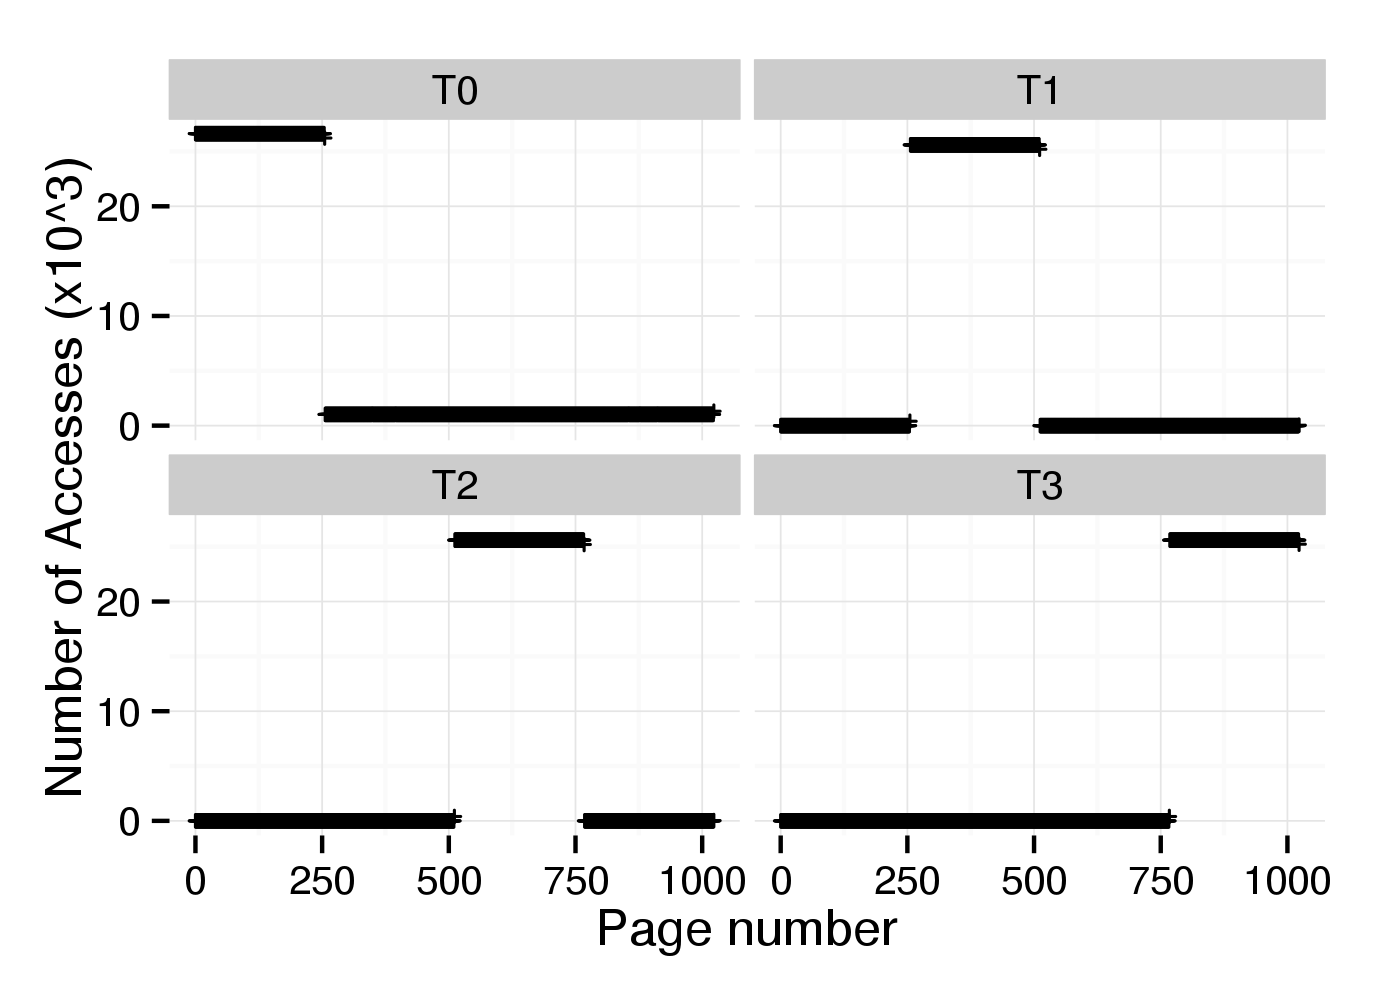
\includegraphics[width=.45\linewidth] {is_w_kba_modif}
        \rule{4cm}{4cm}
        \label{fig:matrix-behaviour-A-naive}
    }
    \subfigure[Structure B (naive)]{
        % 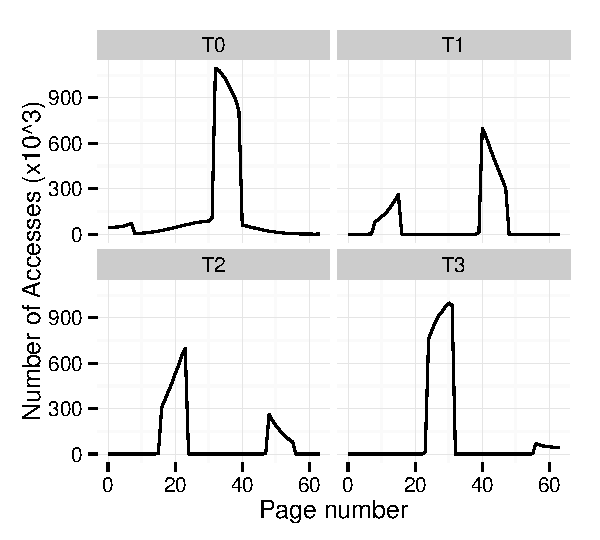
\includegraphics[width=.45\linewidth] {is_w_kb1_modif}
        \rule{4cm}{4cm}
        \label{fig:matrix-behaviour-C-naive}
    }
    \\
    \subfigure[Structure A (bloc)]{
        % 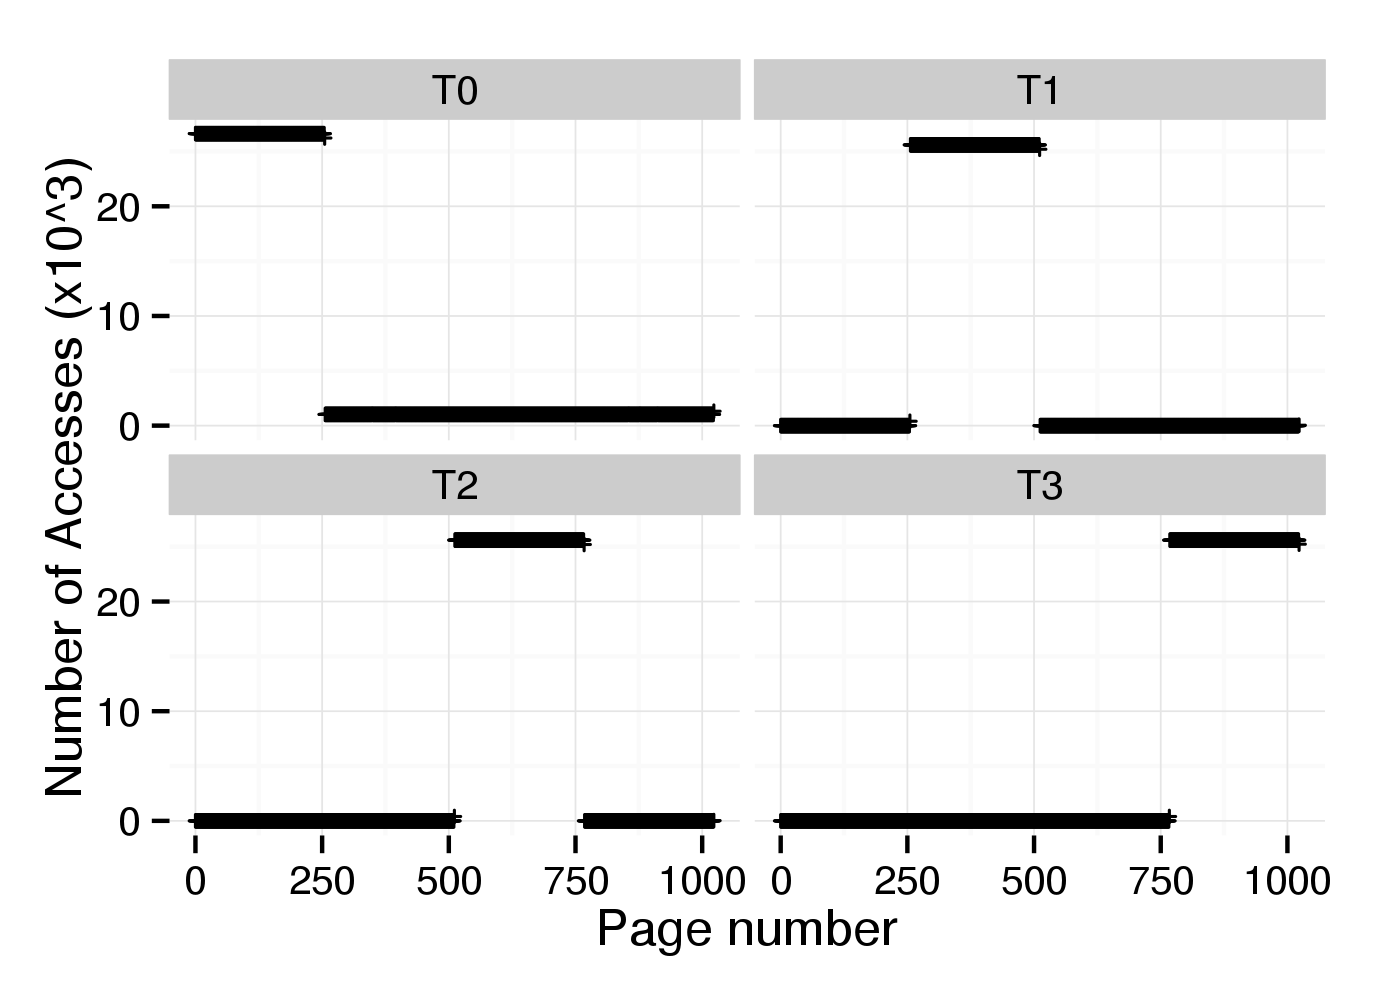
\includegraphics[width=.45\linewidth] {is_w_kba_modif}
        \rule{4cm}{4cm}
        \label{fig:matrix-behaviour-A-bloc}
    }
    \subfigure[Structure B (bloc)]{
        % 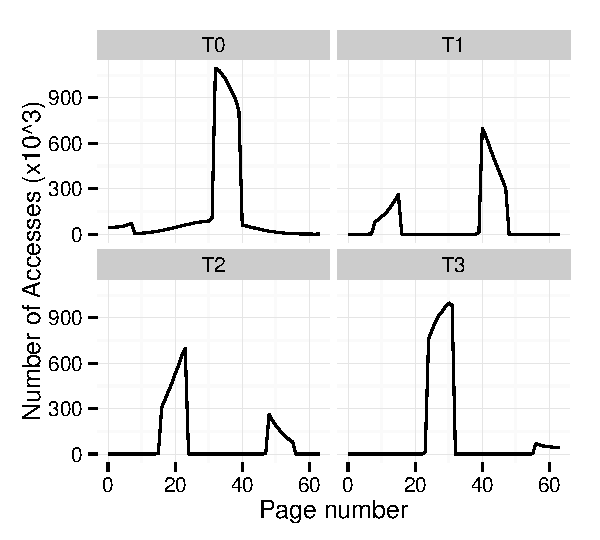
\includegraphics[width=.45\linewidth] {is_w_kb1_modif}
        \rule{4cm}{4cm}
        \label{fig:matrix-behaviour-C-bloc}
    }
    \caption{By thread access distribution on data structures A and B for the
    two matrix multiplications (naive and bloc). Each plots shows the number of access
depending on the page number (inside the structure) for each thread (T0 to
T3).}
    \label{fig:matrix-behaviour}
\end{figure}

Figure \ref{fig:matrix-behaviour} show the thread distribution over the
structures \emph{A}, \emph{B} and \emph{C} for the two implementations of the
\DB{explain the figures}
\begin{itemize}
    \item part of \TABARNAC's output
    \item Different memory patterns
    \item All to all share is bad, \TABARNAC~ warns you, still interleave
        should help
    \item Bloc mapping: all to all unavoidable => interleave, for the other,
        mapping by affinity
\end{itemize}

\begin{figure}[htb]
    \centering
    % \includegraphics{<+file+>}
    \rule{4cm}{4cm}
    \caption{Execution time of the matrix multiplication for size $4096*406$ doubles.}
    \label{fig:matrix-res}
\end{figure}

Results:
\begin{itemize}
    \item Big improvements for naive: better than every other tools
    \item Not that much for Bloc: algo designed to fit in cache figure
        \ref{fig:matrix-res}
    \item Cncl: Tabarnac will help you modify code to do something like naive
        -> bloc if possible or at least to improve your NUMA mapping as for
        naive.
\end{itemize}

